\documentclass{scrbook}

\usepackage[english,ngerman]{babel}
\usepackage[english,ngerman]{babel}
\usepackage[T1]{fontenc}
\usepackage{lmodern}
\usepackage{hyperref}
\usepackage{graphicx}
\usepackage{svg}


\graphicspath{ {./images/} }

\RedeclareSectionCommand[beforeskip=0pt, afterindent=false]{chapter}

\KOMAoptions{%
  paper=a4,
  fontsize=12pt,
  parskip=half,
  headings=normal,
  BCOR=1cm,
  headsepline,
  DIV=12
}

\usepackage{listings}
\usepackage{color}
\usepackage{scrhack}

\definecolor{dkgreen}{rgb}{0,0.6,0}
\definecolor{gray}{rgb}{0.5,0.5,0.5}
\definecolor{mauve}{rgb}{0.58,0,0.82}

\hbadness=4000
\vbadness=2500

\lstset{frame=tb,
  language=Java,
  aboveskip=3mm,
  belowskip=3mm,
  showstringspaces=false,
  columns=flexible,
  basicstyle={\small\ttfamily},
  numbers=none,
  numberstyle=\tiny\color{gray},
  keywordstyle=\color{blue},
  commentstyle=\color{dkgreen},
  stringstyle=\color{mauve},
  breaklines=true,
  breakatwhitespace=true,
  tabsize=3
}



  
\usepackage{cite}
\usepackage[acronym]{glossaries}


\makeglossaries
\newglossaryentry{osgi}
{
    name=OSGi,
    description={Die OSGi Alliance spezifiziert eine hardwareunabhängige dynamische Softwareplattform, die es erleichtert, Anwendungen und ihre Dienste per Komponentenmodell zu modularisieren und zu verwalten}
}

\newglossaryentry{equinox}
{
    name=Equinox,
    description={Equinox ist ein von der Eclipse Foundation entwickeltes Java-basiertes Framework, das die OSGi-Kernspezifikation implementiert}
}

\newglossaryentry{venus}
{
    name=Venus,
    description={Steuerungssoftware der Radargeräte von Thales}
}

\newglossaryentry{buildpipeline}
{
    name=Buildpipline,
    description={Damit werden Anwendungen automatisiert gebaut}
}

\newacronym{mmi}{MMI}{Man Machine Interface}
\newacronym{las}{LAS}{Land and Air Systems}
\newacronym{gsr}{GSR}{Ground and Surface Radars}
\newacronym{stt}{STT}{Single Target Tracking}



\begin{document}
% Vorspann
\frontmatter 
\begin{titlepage}

\date{30.1.2020}
\author{Marco Schäfer}
\title{Erstellung eines Trainingssimulators für Radargeräte durch Restrukturierung, Modularisierung und Erweiterung einer OSGi-Anwendung}
\maketitle

\end{titlepage}

\tableofcontents
\printglossaries

% Hauptinhalt
\mainmatter
\chapter{Einleitung}

\section{Themenumfeld}
Softwaresysteme sind heutzutage im ständigen Wandel und werden insbesondere, seitdem es die Möglichkeit gibt Updates und Patches über das Internet bereitzustellen, immer langlebiger. Wenn Quellcode eine lange Lebensdauer haben soll, ist es unabdingbar, dass dieser eine gute Wartbarkeit hat. Ansonsten können der Zeitaufwand und die Entwicklungskosten bis ins Unermessliche steigen. Diese Kosten entstehen, wenn Fehlerbehebungen am Code durchgeführt werden oder dieser um funktionelle Features erweitert wird. Ein wichtiges Konzept, um die Wartbarkeit von Softwaresystemsen zu verbessern ist eine Modularisierung der Softwarekomponenten.

Im Rahmen der Bachelorarbeit wird eine Anwendung mit einer modularen Architektur entworfen und implementiert. Um dies umzusetzen wird das Framework Equinox verwendet, welches die OSGi-Kernspezifikationen implementiert. „OSGi bietet ein Konzept zur Modularisierung und Komponentisierung von Java-Applikationen, und zwar nicht nur zur Entwicklungszeit, sondern auch zur Laufzeit“. Diese Applikation entsteht bei der Firma Thales Deutschland GmbH am Standort in Ditzingen in der Abteilung LAS (Land and Air Systems). In der Abteilung werden Radarsysteme für den zivilen, wie den militärischen Einsatz entwickelt.  Die Abteilung ist in das Sensorteam und das Venusteam aufgeteilt. Das Venusteam ist für die Steuerungssoftware der Radarsensoren verantwortlich. Die Steuerungssoftware heißt Venus und bietet ein MMI (Man Machine Interface) zur Steuerung von verschiedenen Radargeräten. Zudem visualisiert die Venus Sensordetektionen auf einer Karte und liefert weitere relevante Sensorinformationen, wie z.B. Hardwarefehlermeldungen in Tabellen. Die Software läuft auf einem Laptop und ist über einen speziellen Anschluss mit dem Sensor verbunden.  Zusätzlich entwickeln sie weitere Eclipse Applikationen zum Warten und Testen der Radarsensoren. Das Sensorteam entwickelt die Hardware und Software der verschiedenen Sensormodelle.

\section{Aufgabenstellung}

Das Sensorteam will einen Trainingssimulator erstellen, um neuen Benutzern die Funktionalitäten der Venus näher zu bringen. Bei der Trainingssimulation nehmen ein Trainer und ein bis mehrere Trainees teil. Jeder der beteiligten Personen verfügt über ein Laptop mit der entsprechenden Software. Während der Trainingssimulation, gibt der Trainer Simulationsdaten in die Benutzeroberfläche der Trainingssimulator Anwendung ein. Diese Informationen werden über eine Netzwerkschnittstelle an die Computer der Trainees übermittelt und dort in Echtzeit simuliert. Die Aufgabe des Trainingssimulators ist es, dass die Trainees lernen, die simulierten Daten mit der Steuerungssoftware korrekt zu erfassen und richtig interpretieren. Ein detaillierterer Ablauf wird in Kapitel X.X beschrieben.

Das Ziel dieser Bachelorarbeit ist es, die beschriebene Trainingssimulator Anwendung zu implementieren. Um Wiederverwendbarkeit der Komponenten und eine einfache Erweiterung um funktionelle Features zu gewährleisten, steht eine modulare Architektur der Software im Vordergrund. Die Grundlage für diese Anwendung ist ein Radarsimulator, welcher einen realen Radarsensor simuliert. Dieser Radarsimulator wurde von früheren Praktikanten und Werkstudenten programmiert und wird derzeitig für interne Tests der Venus verwendet. Jedoch tendiert die Softwarearchitektur des Radarsimulators zu einer monolithischen Architektur, da einzelne Softwaremodule mehrere verschiedene Funktionen haben und wenig klare Schnittstellen zwischen den bereits vorhandenen Modulen definiert sind. Damit darauf sinnvoll aufgebaut werden kann, muss diese Architektur im Vorhinein überarbeitet werden. Zudem soll die Anwendung so angepasst werden, dass der Großteil der Softwarekomponenten in der Testanwendung und in der Trainingssimulator Anwendung verwendet werden können. Dazu muss eine entsprechende Architektur erstellt werden, die durch möglichst wenige Änderungen zu den verschiedenen Ausprägungen abgeleitet werden kann.

Eine weitere Aufgabe ist es, die Trainingsanwendung, sowie die Testanwendung und um drei Features ergänzt werden. Diese Features sind Single Target Tracking, die Bereitstellung des Dopplertons während STT und die Einbindung der Detektionswahrscheinlichkeit von Radarobjekten. Single Target Tracking ist die Funktion ein Radarziel über einen bestimmten Zeitraum zu verfolgen. Dabei wählt man ein bereits existierendes Ziel in der Venus aus und startet den STT Modus. Daraufhin schwenkt der Sensor mit einem kleinen Winkel über das Ziel und richtet sich bei Bewegung des Zieles neu aus. Diese Funktion wird vom Sensor bereitgestellt und nicht von der Venus. Deshalb muss der Simulator diese Funktion bereitstellen. Wenn das Ziel von STT erfasst wird soll nun der Dopplerton des verfolgten Objektes per Audio abgespielt werden. *Detektionswahrscheinlichkeit* Diese Features sollen eine realistischere Trainingsumgebung für neue Nutzer des Trainingssimulators bieten.


\section{Aufbau der Thesis}
Zu Beginn der Thesis werden die allgemeinen Grundlagen der Konzepte und Technologien, die in dieser Arbeit verwendet werden, erläutert. Als nächstes wird die alte Architektur des Radarsimulator analysiert und auf Schwachstellen überprüft. Zudem werden die funktionellen Anforderrungen der Trainingssimulator- und Testsimulatorandwendung aufgelistet und es wird untersucht an welchen Komponenten die vorgegebenen Erweiterungen anknüpfen müssen. Nach der Analyse wird das Konzept der neuen Architektur vorgestellt. Ein besonderes Augenmerk wird dabei auf die Softwaremodule und deren Schnittstellen gelegt. Des Weiteren werden den verschiedenen Anwendungsausprägungen die Softwaremodule zugeordnet und genauer erklärt. Außerdem wird gezeigt, wie das Datenmodell verändert wurde und von den neuen Softwarekomponenten verwendet wird. Ergänzend wird darauf eingegangen, wie die Buildpipline die Testanwendung, die Traineranwendung und die Traineeanwendung baut. Im folgenden Kapitel wird erklärt, wie die Softwarekomponenten implementiert und zusammengesetzt wurden. Danach wird bewertet, wie der Status der Applikation am Ende des Projektes aussieht, bzw. ob alle wichtigen Funktionen enthalten sind und die Anwendung stabil läuft. Zuletzt gibt es noch eine Schlussbetrachtung der Thesis, in der Erkenntnisse der Arbeit beschrieben werden und wie es in der Zukunft mit den Technologien und der Anwendung weitergehen soll.

\chapter{Grundlagen}
\section{Softwarearchitektur}
\subsection{Modulare Software}
TODO
\subsection{Model-Driven-Architecture}
TODO
\section{OSGi}
TODO
\section{Radarsimulator}
TODO
\subsection{Venus}
TODO
\chapter{Analyse}

\section{Anforderungsanalyse der Ausprägungen/Anwendungen}
\subsection{Funktionale Anforderungen}

In diesem Abschnitt werden die funktionalen Anforderungen der drei Anwendungen, die im Rahmen dieser Arbeit entstanden sind, vorgestellt.
Funktionale Anforderungen beschreiben gewünschte Funktionalitäten (was soll das System tun/können) eines Systems bzw. Produkts, dessen Daten oder
Verhalten\cite{funkAnf}.

Die funktionalen Anforderungen des Trainersimulators sind:

\begin{itemize}
    \item Der Trainersimulator muss dem Trainee ermöglichen sich mit ihm zu verbinden, wenn dieser sich im selben Netzwerk befindet und die korrekte IP-Adresse hat.
    \item Der Trainersimulator muss bei Änderungen von PNU-Daten, beim Hinzufügen von Bitfehlern oder dem Abspielen von Szenarien durch die graphische Oberfläche, die entsprechenden Informationen über das Netzwerk an alle verbundenen Trainees übertragen.
\end{itemize}

Der Traineesimulator hat folgende funktionale Anforderungen:
\begin{itemize}
    \item Der Traineesimulator soll sich mit dem Trainersimulator verbinden können.
    \item Der Trainingssimulator soll sich mit der Venus verbinden, nachdem dieser die nötigen Informationen vom Trainersimulator empfangen hat.
    \item Der Trainingssimulator muss, wenn er Simulations-Daten vom Trainersimulator empfängt, diese verarbeiten und über das Asterix-Interface versenden.
\end{itemize}

Die funktionalen Anforderungen der Testanwendung sollen nicht von den funktionalen Anforderungen des Radarsimulators nicht abweichen. Diese lauten:

\begin{itemize}
    \item Der Testsimulator soll eine Verbindung zur Venus über das Asterix-Interface aufbauen
    \item Der Testsimulator muss Informationen, die auf der graphischen Benutzeroberfläche verändert wurden, über das Asterix-Interface versenden.
\end{itemize}

\subsection{Nicht funktionale Anforderungen}

Nichtfunktionale Anforderungen sind Anforderungen, an die Qualität in welcher die geforderte Funktionalität zu erbringen ist \cite{funkAnf}. Die nicht funktionalen Anforderungen lassen sich für die drei Applikationen zusammenfassen, da diese fast vollständig übereinstimmen. Lediglich durch die Netzwerkverbindung der Trainer- und Traineeanwendung entstehen Unterschiede. Die nichtfunktionalen Anforderungen lassen sich in mehrere Bereiche unterteilen. Leistungsanforderungen, Qualitätsanforderungen und Randbedingungen.

Unter Leistungsanforderungen versteht man im Allgemeinen, Anforderungen an die empirisch messbaren nicht-funktionalen Anforderungen eines Systems, also
Anforderungen, deren zu Grunde liegendes Bedürfnis ein Leistungsmerkmal ist.\cite{nFunkAnf}. Eine Leistungsanforderung jeder Anwendung ist, dass diese die Simulation in Echtzeit ausführt und eine Verzögerung um 10 ms im akzeptablen Bereich liegt. Zudem sollen diese nicht zu viel Speicher besetzen und die Prozessorbelastung sollte einen realistischen Wert betragen. Um dafür zu garantieren werden Belastungstests, mit der entsprechenden Hardware, auf der die Anwendung später laufen soll, durchgeführt.

Um die Qualitätsanforderungen zu überprüfen wird der ISO/IEC 25010 verwendet. Der ISO/IEC 25010 \cite{iso25010}Software engeneering Software product Qualitiy Requirements and Evaluation (SQUuarRE) ist ein aktueller Standard für die Qualitätskriterien und -bewertungen von Softwareprodukten. Der Software Product Quality Model aus dem Standard ISO/IEC 25010 beschreibt acht Kriterien, um die Qualität eines Produktes zu bewerten. Die acht Kriterien sind:
\begin{itemize}
    \item Funktionalität
    \item Leistungseffizienz
    \item Kompatibilität
    \item Benutzbarkeit
    \item Zuverlässigkeit
    \item Sicherheit
    \item Wartbarkeit
    \item Übertragbarkeit
\end{itemize}

Die Qualitätsanforderung, die in dieser Arbeit im Mittelpunkt steht, ist die Wartbarkeit. Die Unterpunkte im Bereich Wertbarkeit des ISO 25010 sind Modularität, Wiederverwendbarkeit, Analysierbarkeit, Modifizierbarkeit und Testbarkeit. Wie bereits erwähnt, soll die Arbeit genau diese Kriterien beachten. 

In Bezug auf die Modularität, soll eine Anwendung aus losen Komponenten bestehen, bei denen wichtig ist, dass diese Möglichst wenig Abhängigkeiten haben. Dies wird durch gut definierte Schnittstellen erreicht und hat den Vorteil, dass Änderungen der Module minimale Auswirkungen auf das Gesamtsystem haben. Um die Modularität der Anwendung weiter zu verbessern wird das OSGi-Framework \Gls{equinox} verwendet.
Wiederverwendbarkeit spielt eine besondere Rolle, da in dieser Arbeit gleich drei Anwendungen erstellt werden. Man erkennt gute Wiederverwendbarkeit von Code, wenn es wenig, bis keinen redundanten Code zwischen den Anwendungen gibt. Die Analysierbarkeit des Systems wird darin gemessen, wie gut erkannt werden kann, was durch die Änderung einer Komponente mit dem Gesamtsystem passiert. Außerdem hängt sie davon ab, wie gut sich fehlerhafte Komponenten erkennen lassen. Wenn ein System einfach geändert werden kann, ohne das Defekte entstehen, dann hat es gute Modifizierbarkeit. Da die drei Anwendungen auch von neuen Mitarbeitern weiterentwickelt werden, sind eine gute Analysierbarkeit und eine gute Wartbarkeit notwendig.  Dadurch können die Einarbeitungszeit und der Weiterentwicklungsaufwand deutlich gesenkt werden.

Des Weiteren soll die Anwendung einfach testbar sein. Dies wird auch durch die Modularisierung der Systemkomponenten erreicht. Diese lassen sich einzeln gut Testen und lassen sich gut mocken, damit diese Mocks in die weiteren Tests eingebunden werden.

Die Funktionalität ist in den funktionalen Anforderungen angegeben und kann, wie die Benutzbarkeit, durch manuelle Tests überprüft werden. Die Leistungseffizienz und die Zuverlässigkeit der Anwendung kann über Langzeittests überprüft werden. Diese Anforderungen sind nicht vollständig zu vernachlässigen, aber sie müssen bei den Anwendungen die im Rahmen der Bachelorarbeit entstehen, nur in einem geringen Maße erfüllt werden. Das Ziel ist es die Anwendung auszuführen, ohne das drastische Bedienungs- und Performanceprobleme auftreten.

Die Sicherheit, die Übertragbarkeit und die Kompatibilität sind zu vernachlässigen, da die Anwendung auf festgelegter Hardware läuft und diese keinen Zugang zum Internet hat. 

\newpage
\section{Analyse des Radarsimulators}

\subsection{Softwarearchitektur}

Im folgenden Abschnitt werden die einzelnen Softwarekomponenten der Radarsimulator Anwendung beschrieben und auf Wiederverwendbarkeit und Modularität überprüft. Dabei stehen die Kernkomponenten der Anwendung im Fokus. Der Radarsimulator wird von Thales zur Verfügung gestellt und wurde vor und während dem Schreiben des Kapitels nicht verändert. Der Radarsimulator mit neuer Architektur wird in den folgenden Kapiteln Testsimulator genannt.

Der Radarsimulator ist eine Eclipse-RCP Anwendung und setzt sich aus mehreren Equinox Plug-In-Modulen zusammen. Er wird durch Basis-Plug-Ins der Venus unterstütz. Diese stellen spezifische Funktionen, wie Anwendungsstruktur und Helferklassen zur Verfügung. Der Startpunkt der Anwendung ist die Klasse \texttt{SimulatorMain}, welche sich in dem Modul \texttt{RadarSimulator.app} befindet. Dieses stellt die Benutzeroberfläche des Simulators zur Verfügung. Im Modul werden die Startklasse der Anwendung und weitere Fenstereinstellungen für diese Anwendungen in einer \texttt{Application.e4xmi-Datei} angegeben. Diese Datei ist die Basis jeder Eclipse-RCP Applikation. Wenn die Eclipse Applikation die Startklasse in Java aufruft, startet der RestartService. Diese ist im folgenden Codeabschnitt zu sehen.


\begin{lstlisting}

@PostConstruct
void start(final BorderPane parent) {
    this.parent = parent;
    restartService.setOnScheduled(e -> {
        parent.setCenter(new JFXSpinner());
        disposeOverview();
    });
    restartService.setOnSucceeded(e -> {
        instance = restartService.getValue();
        initSimulatorOverview(instance);
    });
    restartService.restart();
}

\end{lstlisting}


Die gesamte Funktionalität der Sensorsimulation stellt die \texttt{SimulatorInstance zur Verfügung}. Wenn der \texttt{RestartService} die \texttt{SimulatorInstance} erfolgreich geladen hat, initialisiert dieser die Benutzeroberfläche der Anwendung. Außerdem ermöglicht es der \texttt{RestartService}, die Simulation durch einen Mausklick in ein Fenster Menü item neu zu starten. Dabei werden die Benutzeroberfläche, sowie die \texttt{SimulatorInstance} neu geladen. Der \texttt{RestartService} soll zudem auch im zukünftigen Testsimulator sowie im Trainer- und Traineesimulator enthalten sein. Die \texttt{SimulatorInstance} und der \texttt{SimulatorMainContentProvider} werden in der SimulatorMain als Attribute gespeichert. Wenn die Benutzeroberfläche geladen wird, bekommt diese die \texttt{SimulatorInstance} übergeben, damit diese die Simulation steuern kann. Wie es bei einer Eclipse Applikation üblich ist, sind Funktionen der Anwendung in Softwaremodule eingeteilt. Diese Module heißen im Equinox-Framework Plug-Ins. Auf Abbildung \ref{img:SimulatorModels} erkennt man die Aufteilung der Hauptkomponenten in zwei Plug-Ins.

\begin{figure}[h]
    \centering
    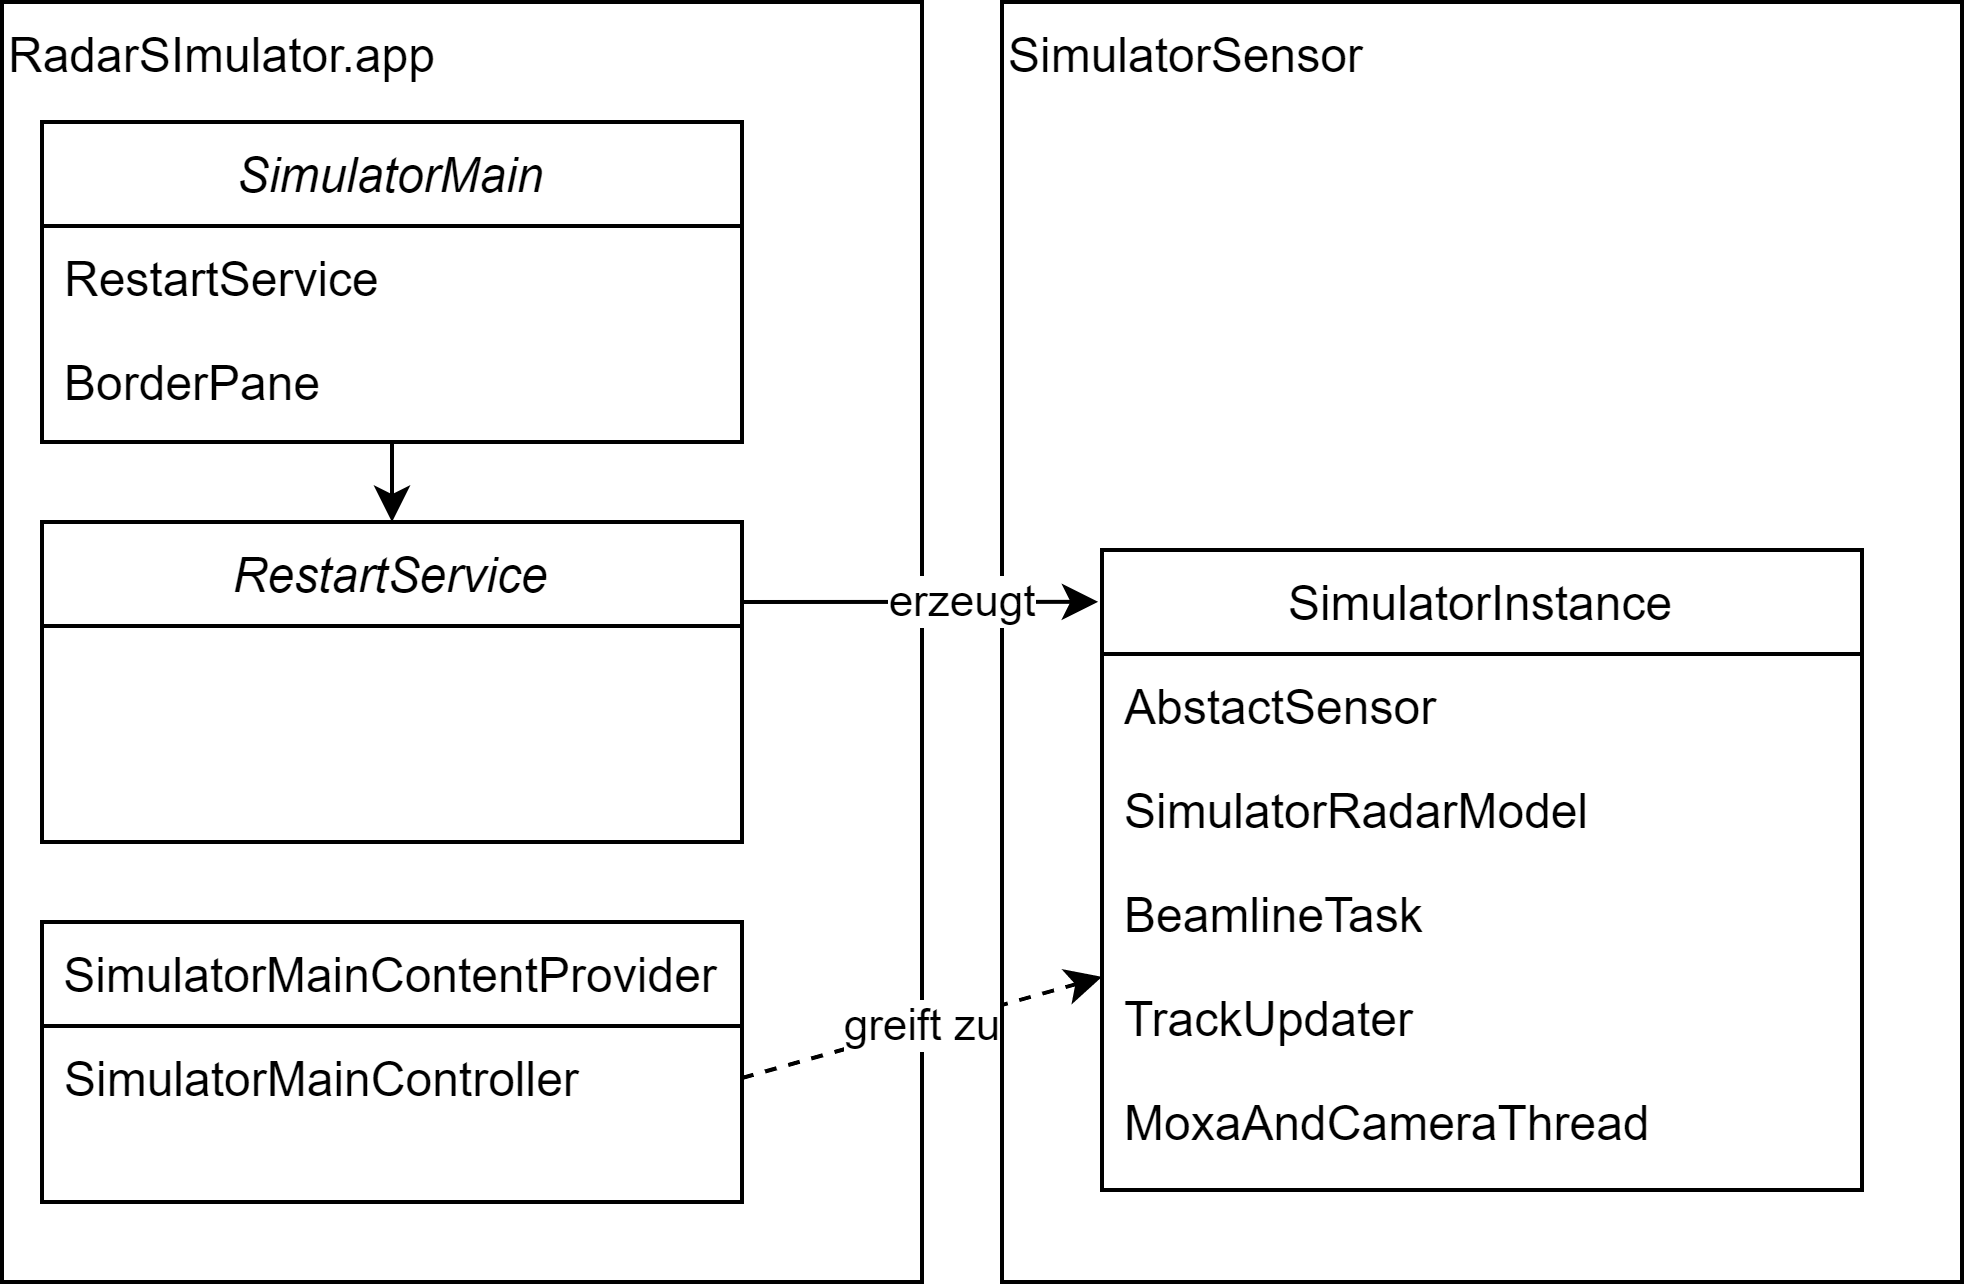
\includegraphics[width=0.8\textwidth]{content/assets/Kapitel3/SimulatorModels.png}
    \caption{Die Module \texttt{SensorSimulator} und \texttt{RadarSimulator.app} des Radarsimulators}
    \label{img:SimulatorModels}
\end{figure}

\input{content/Analyse/benutzeroberfläche}
\subsection{SimulatorInstance}
Die SimulatorInstance hat folgende Aufgaben:
\begin{itemize}
    \item Erstellen des Datenmodells des Simulators. Aufgrund von unterschiedlichen Werten und Zubehör zwischen den Sensortypen, wird das Datenmodell je nach Sensortyp und Asterix-version entsprechend befüllt. Dafür wird eine Helferklasse verwendet.
    \item Erstellen eines Sensors, je nach Sensortyp wird ein passender Sensor initialisiert. 
    Der AbstractSensor ist die Vaterklasse der jeweiligen Sensortypen (\texttt{SensorBORA}, SensorGO12, SensorGO80 und SensorGA10). Über den Sensor können \\Asterix-Kommandos an die Venus versendet werden
    \item Erstellen und starten des BeamlineTasks. Der BeamlineTask ist dafür zuständig, dass sich die Beamline des Sensors korrekt bewegt und die entsprechenden Werte im Modell geupdatet werden.
    \item Erstellen und starten des Trackupdater. Er ist dafür zuständig die Tracks korrekt upgedatet werden und über das Asterixinterface versendet werden.
    \item Erstellen und starten des MoaxaAndCameraServerTask. Dieser simuliert optionales Zubehör und die Kamera, falls dieser vorhanden ist.    
    
\end{itemize}

Diese Tasks haben eine klar definierte Aufgabe und lassen sich gut wiederverwenden.
\subsection{Model}


Das Datenmodell des Radarsimulators wird mithilfe des Frameworks EMF erstellt. Das Modell befindet sich in einem eigenen Plug-In Modul. Darin sind ein graphisches Entity-Relation-Diagramm des Modells und der daraus generierbare Modellcode enthalten. Das Objekt, welches die Informationen des Sensors zusammenfasst, heißt SimulatorModelRadar. Dieses enthält 19 Attribute, die die Eigenschaften des simulierten Sensors beschreiben. Zusätzlich gibt es noch Beziehungen zu zehn Klassen, die die Daten des Sensors speichern. 

Die Klassen, die in dieser Arbeit verwendet werden, sind:

\begin{itemize}
    \item SimulatorBitNode: Der SimulatorBitNode ist eine Baumdatenstruktur in der Bitfehler abgelegt werden. Das SimulatorModelRadar besitzt höchstens einen SimulatorBitNode.
    \item SimulatorModelEquipment: Der SimulatorModelRadar kann beliebig viele   \\
    SimulatorModelEquipment-Objekte des Sensors gespeichern. Weil die PNU ein Zubehör des Sensors ist, werden dessen Informationen als SimulatorModelEquipment gespeichert. Dafür gibt es eine Klasse, welche SimulatorModelEquipment erweitert. Diese heißt SimulatorModelPNU.
    \item SimulatorModelSector: Um Sektor Informationen des Sensors zu speichern, gibt es die Klasse SimulatorModelSector. Die Klasse SimulatorModelRadar hat höchstens einen aktuellen Sektor und beliebig viele weitere Sektoren.    
\end{itemize}

Was bei der Betrachtung des grafischen Modells auffällt ist, dass es drei vom SimulatorModelRadar unabhängige Klassen gibt. Diese Klassen sind:

\begin{itemize}
    \item \texttt{Scenario}: Die Klasse Scenario beinhaltet beliebig viele ScenarioTargets, welche beliebig viele Waypoints haben. Man erkennt daran gut wie das Scenario aufgebaut ist. Die ScenarioTargets sind mögliche Objekt, die der Sensor detektieren kann. Das sind zum Beispiel Fußgänger oder PKWs. Diese Objekte bewegen sich auf einem Pfad, welcher durch die Waypoints (auf Deutsch Wegpunkte) definiert wird.
    \item \texttt{TargetSimulation}:  Die TargetSimulation beschreibt die Eigenschaften, wie z.B. Position, Klassifizierung und Radarquerschnitt, eines Radarziels zu einem bestimmten Zeitpunkt. Eine TargetSimulation entsteht, wenn im UI ein Scenario abgespielt wird. Dabei wird die aktuelle Position eines ScenarioTargets, anhand der Wegpunkte berechnet und daraus wird eine TargetSimulation erstellt.
    \item SimulatorModelTrack: Ein SimulatorModelTrack beschreibt ebenso, wie die TargetSimulation, die Eigenschaften eines Radarziels. Der entscheidende Unterschied ist, dass dieses Radarziel nun abhängig vom Sensor ist. Deswegen hat dieser weitere Attribute, welche die Venus benötigt um das Ziel darzustellen. In Tabelle \ref{table:1} werden die entscheidenden Unterschiede der beiden Klassen aufgezeigt.    
\end{itemize}

\begin{table}[h]
    \begin{tabular}{ |c|c|c| } 
        \hline
         & \texttt{TargetSimulation} & \texttt{SimulatorModelTrack} \\ 
        \hline
        Koordinatensystem & Lat/Long & Polarkoordinaten \\ 
        \hline
        Doppler Speed Informationen & - & x \\ 
        \hline
        
   \end{tabular}
   \caption{Vergleich zwischen\texttt{TargetSimulation} und \texttt{SimulatorModelTrack}}
   \label{table:1}
\end{table}

Wie sinnvoll ist es nun diese Klassen vom Modell zu trennen? Das Scenario wird von der UI Komponente verwendet, um es auf einer Karte darzustellen und um es als XML-Datei zu speichern. Wie man in Abbildung \ref{figure:scenarioview} erkennen kann gehört das Scenario zum ScenarioController und lediglich der ScenarioUpdater ist vo ihm abhängig. Deswegen ist es nicht notwendig das Scenario im Modell zu speichern und es müssen keine Änderungen vorgenommen werden.

\begin{figure}[h!]
    \centering
    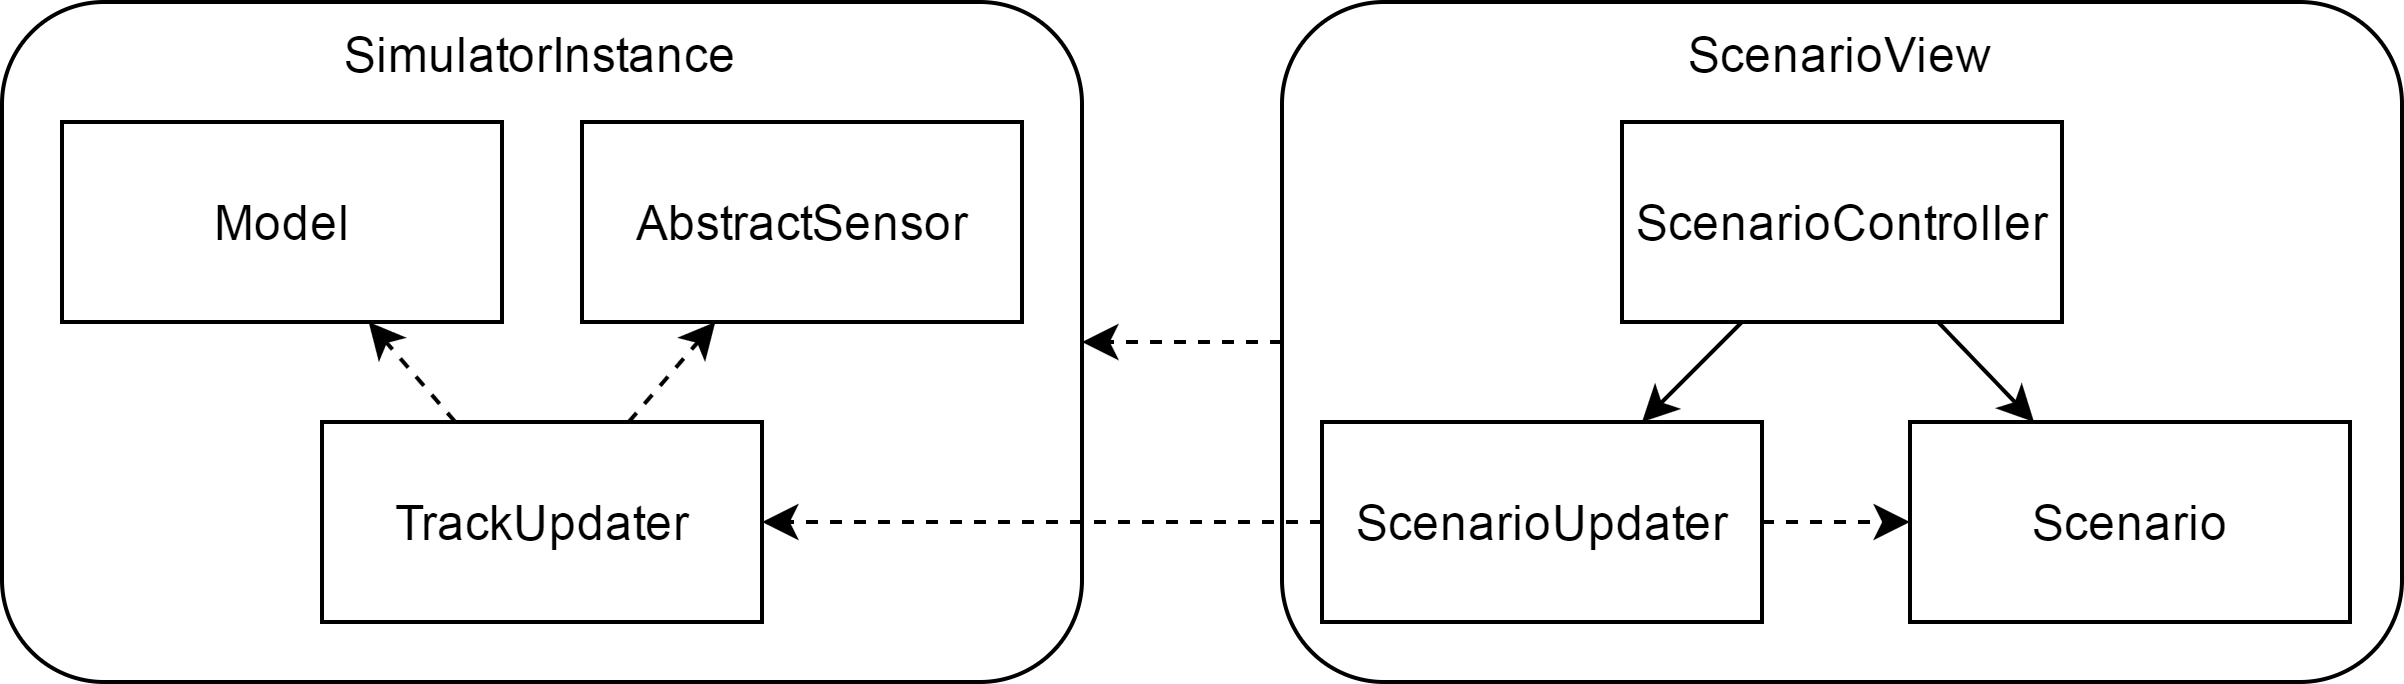
\includegraphics[width=1\textwidth]{content/assets/Kapitel3/ScenarioViewRelations.png}
    \caption{Beziehung zwischen SimulatorInstance und ScenarioView}
    \label{figure:scenarioview}
\end{figure}


\chapter{Konzept}

\section{Neue Architektur}
Die neue Architektur soll eine gute und stabile Basis für alle drei Anwendungen bieten. Das soll durch das Erstellen von modularen Komponenten geschehen. 

Der Kernstruktur der drei Anwendungen soll identisch sein, sodass mit möglichst wenig unterschiedlichem Code notwendig ist um die verschiedenen 
Anwendungen zu erstellen. Bei den Softwaremodulen ist es wichtig, dass diese eine eindeutige Funktion haben, dass eindeutige Schnittstelen definiert sind
 und dass diese gut wiederverwendet werden können. 

\input{content/Konzept/konzeptBenutzeroberfläche}
\subsection{SimulatorInstance}
Die SimulatorInstance unterscheidet sich bei jeder Anwendungsausprägung. Jedoch gibt es Komponenten, welche von mehreren der Anwendungen verwendet werden 
können. Im Folgenden wird die Grundstruktur SimulatorInstance beschrieben, welche Komponenten diese verwenden kann und wie letztendlich die 
unterschiedlichen Instancen aufgeteilt sind.

Eine Komponente, die jede Instance enthält, ist ein Datenmodell. Es wurde entschieden, dass das Modell des RadarSimulators mit einer kleinen Erweiterung,
 für alle drei Anwendungen genutzt wird. Dadurch kann nicht nur der Modell-Code wiederverwendet werden, sondern auch der Code zum Erstellen und Verwalten 
des Modells bleibt identisch.

Da es nun eine Komponente gibt, die jede Anwendungsausprägung verwendet, ist es sinnvoll eine Klasse zu erstellen, die das Modell verwaltet und auf der 
die weiteren Simulator Instanzen aufbauen. Diese Klasse heißt SimulatorCore.





\newpage
\section{Features}

\subsection{Single Target Tracking}
Um Single Target Tracking zu ermöglichen, benötigt die Anwendung eine Erweiterung um zwei Funktionen. Zum einen muss überprüft werden, ob sich ein Ziel 
im Suchbereich befindet, wenn dies zutrifft, soll nach jeder Bewegung des Ziels, das Audiogate auf dessen Position gesetzt werden. Des Weiteren muss sich 
die Beamline, je nach Zielverfolgung oder Zielsuche korrekt verhalten.

Während der STT Modus aktiviert ist, bewegt sich die Beamline innerhalb eines engen Sektors wiederholt über das Ziel. Wenn kein Ziel gefunden wird, sucht
die Beamline in einem größeren Bereich nach einem neuen Ziel. Der Sektor hat das Audiogate als Mittelpunkt und ändert seinen Bereich synchron zum 
Audiogate. Wenn ein Ziel verfolgt wird beträgt die Breite des Sektors 100 mils. Falls der Sensor ein Ziel zur Verfolgung sucht, beträgt die 
Bewegungsweite 300 mils. Diese Funktion wird im BeamlineTask implementiert, da dieser Zugriff auf das Audiogate und die Beamlineinformationen hat. Der 
BeamlineTask hat jedoch keinen Zugriff auf die Daten der Tracks. Deshalb weiß er nicht, ob ein Ziel verfolgt wird und kann kein Audiogate setzen. Damit 
der Beamlinetask weiß, ob ein Ziel verfolgt wird, wird ein Booleanflag, welches jederzeit abgefragt werden kann, im Model hinzugefügt.

Das Flag, sowie das Audiogate sollen vom Trackupdater gestetzt werden. Dieser hat alle Informationen der verfügbaren Tracks, die in der Simulation 
existieren und kann berechnen, ob das Ziel derzeitig von der Beamline erfasst wird. Der TrackUpdater hat die Methode schedule(), welche wiederholt nach 
einem bestimmten Zeitintervall aufgerufen wird. Diese Methode aktualisiert die Tracks und sendet Track Informationen an den Sensor. Diese Methode wird 
nun erweitert, um das STTFlag und das Audiogate zu setzen. Ein verfolgter Track wird im TrackUpdater gespeichert.

Zum Anfang der Methode wird überprüft, ob bereits ein Track verfolgt wird, falls dies nicht der Fall ist wird die Distanz vom Audiogate zu allen 
vorhandenen Tracks berechnet. Die Werte werden in einer Liste mit dem jeweiligen Track gespeichert, wenn sie innerhalb des STT-Sektors liegen. Die 
STT-Funktion ist so definiert, dass sie den nächsten Track zum Audiogate innerhalb des Sektors so lange verfolgt, bis dieser verschwindet oder man das 
Audiogate manuell ändert. Deshalb wird die Liste so sortiert, damit der Track mit dem geringsten Abstand zum Audiogate an erster Stelle steht. Nachdem 
sortiert wurde, wird das erste Element gespeichert, das Flag wird auf true gesetzt und die Liste wird geleert. Wenn die Liste leer ist wird nichts getan. 

Wird bereits ein Track verfolgt, wird geprüft, ob der zu verfolgende Track aktuell existiert. Das passiert indem man in der Liste, der gegenwärtigen 
Tracks nach einem Track mit der identischen ID des gespeicherten Tracks ist sucht. Ist dieser vorhanden, wird dieser Track als neuer Track gespeichert. 
Als nächstes wird getestet, ob dieser Track vom Sensor detektiert wird.  Trifft es zu, dass der Track vorhanden ist und detektiert wird setzt der 
TrackUpdater das Audiogate auf die aktuelle Position des Tracks. Wenn der Track nicht detektiert wird oder existiert, wird ein Zähler hochgezählt. Es 
kann passieren, dass ein Track in einem oder mehreren Durchläufen nicht im Bereich der Beamline liegt oder dass der Track vom Sensor nicht erfasst wird, 
da er z.B. zu weit entfernt ist. Durch den Zähler kann man einen Toleranzwert festlegen, wie oft der Track nicht erkannt werden muss bevor diesem nicht 
mehr gefolgt wird. Dem Track wird entfolgt, indem das Flag auf false gesetzt und der Track gelöscht wird.

\begin{figure}[h]
    \centering
    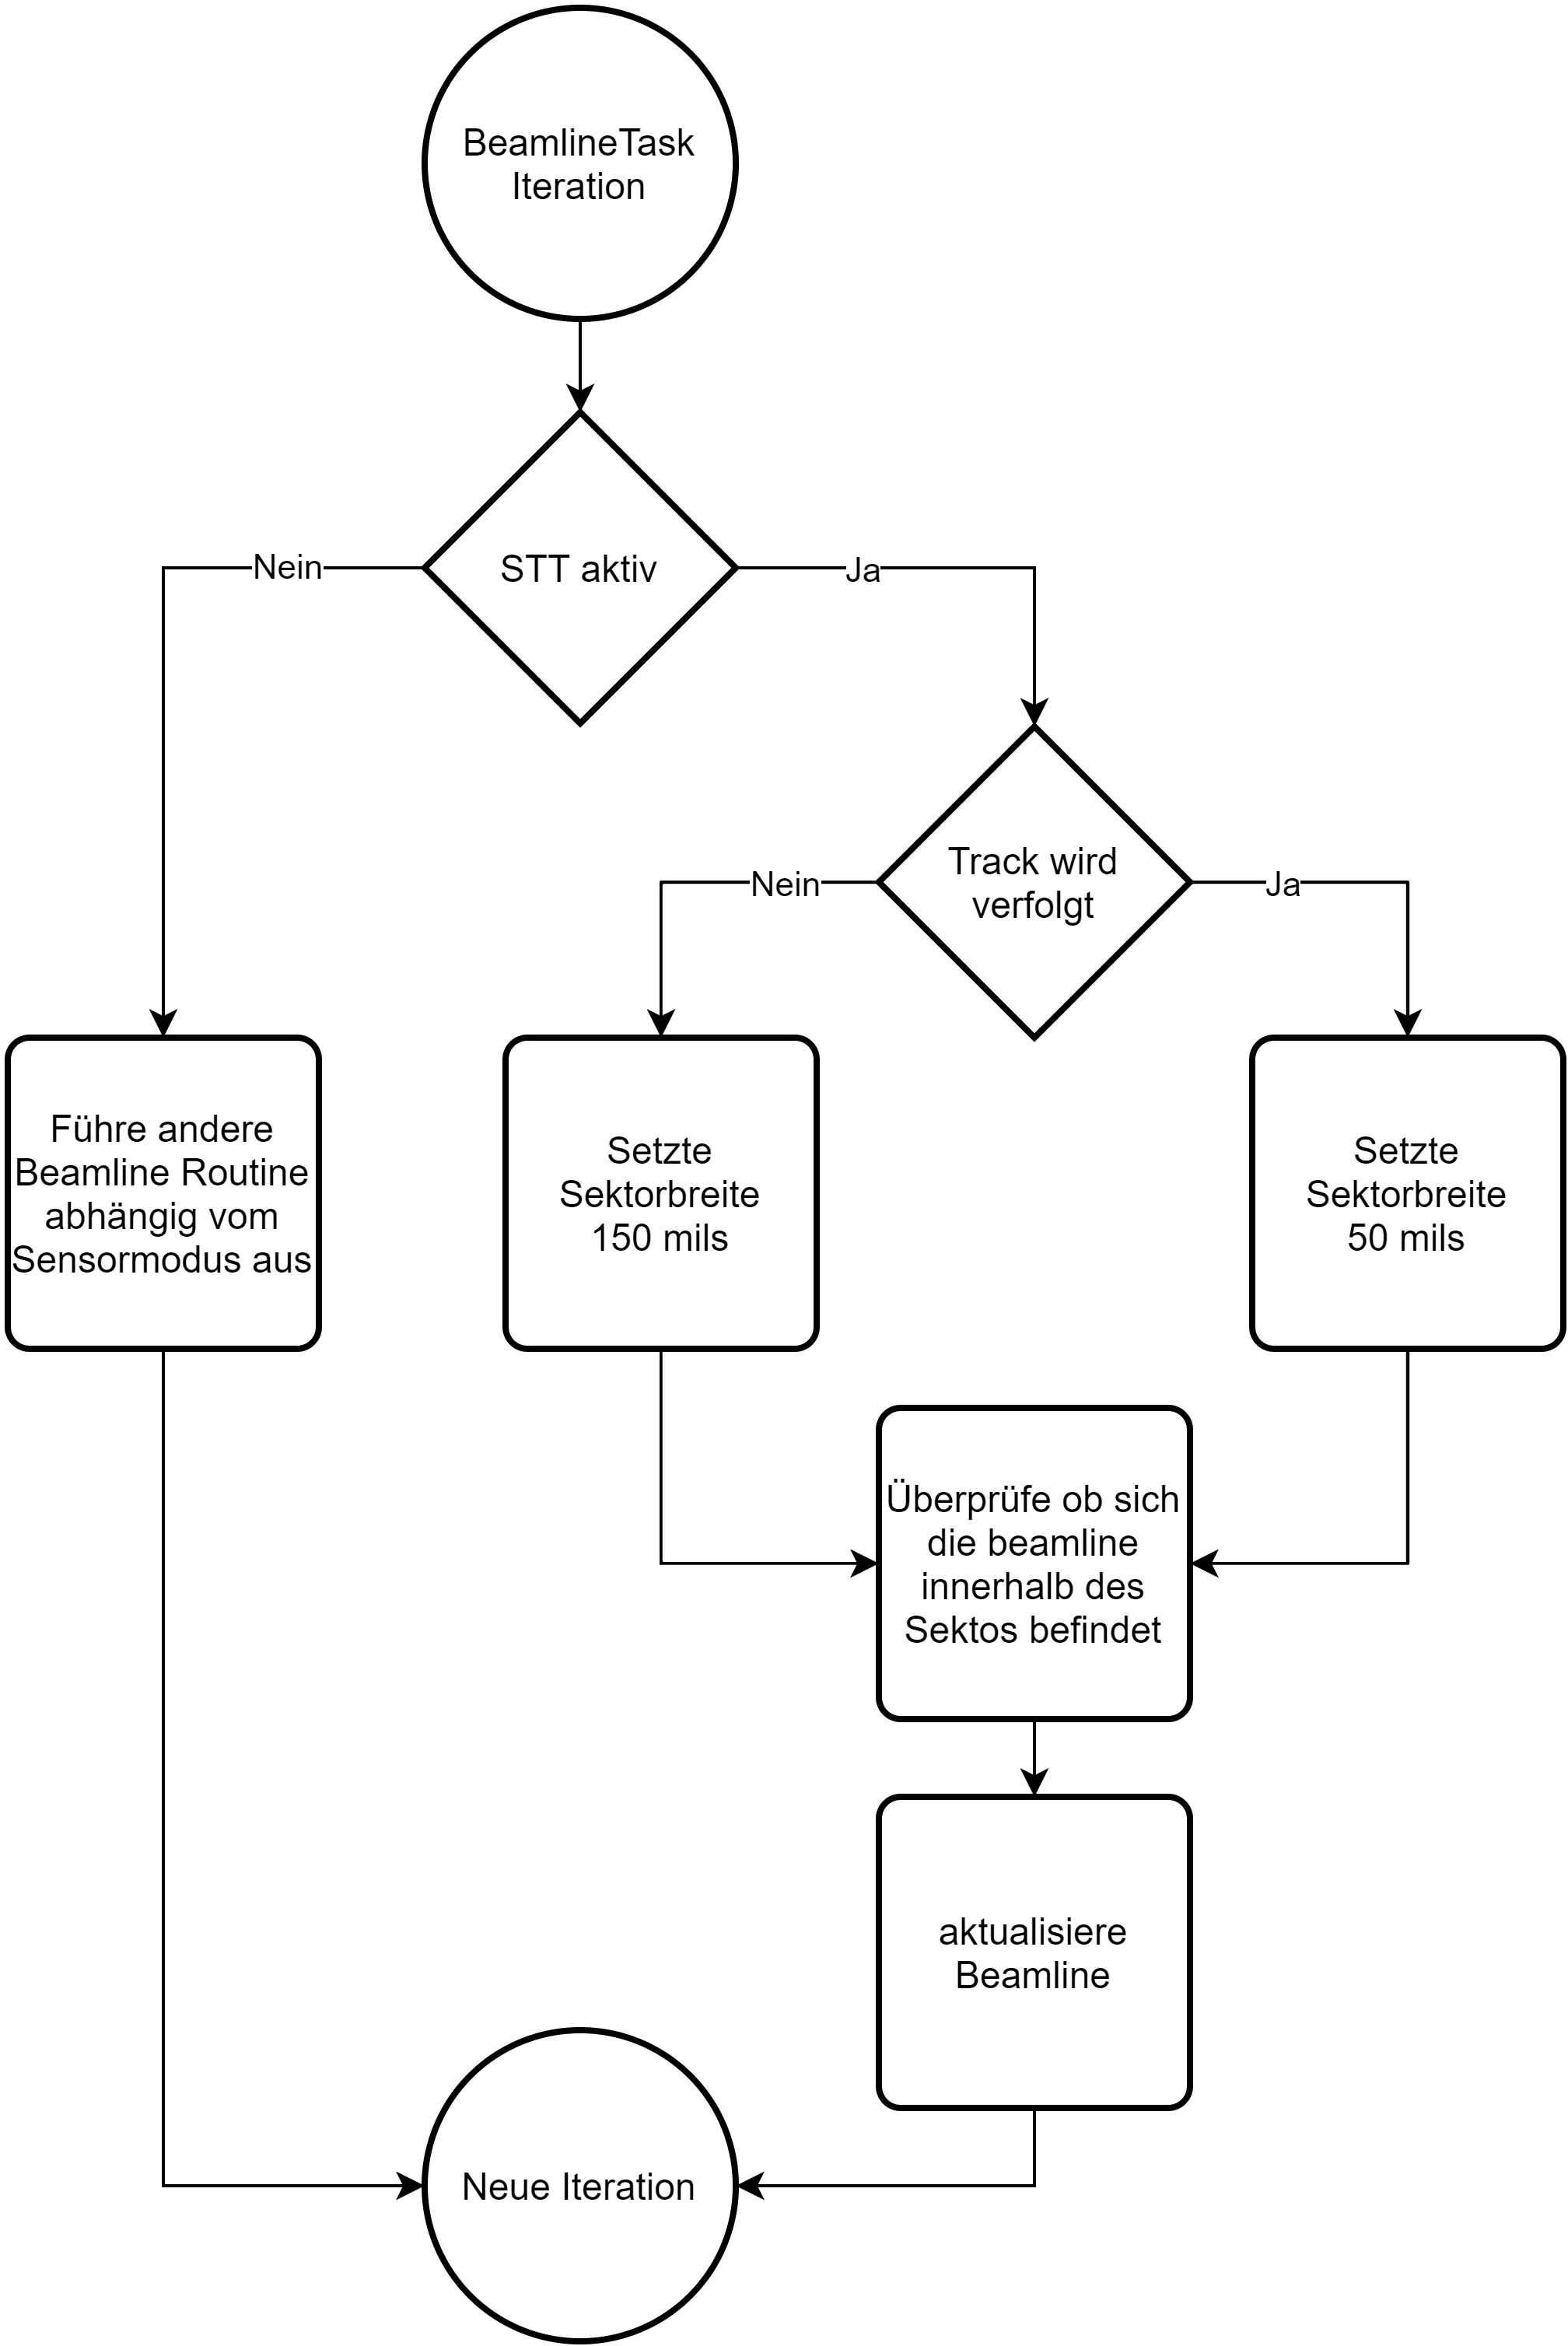
\includegraphics[width=0.6\textwidth]{content/assets/BeamlineTaskSTT.png}
    \caption{Flussdiagramm des Algorithmus des BeamlineTask}
\end{figure}

\begin{figure}[h]
    \centering
    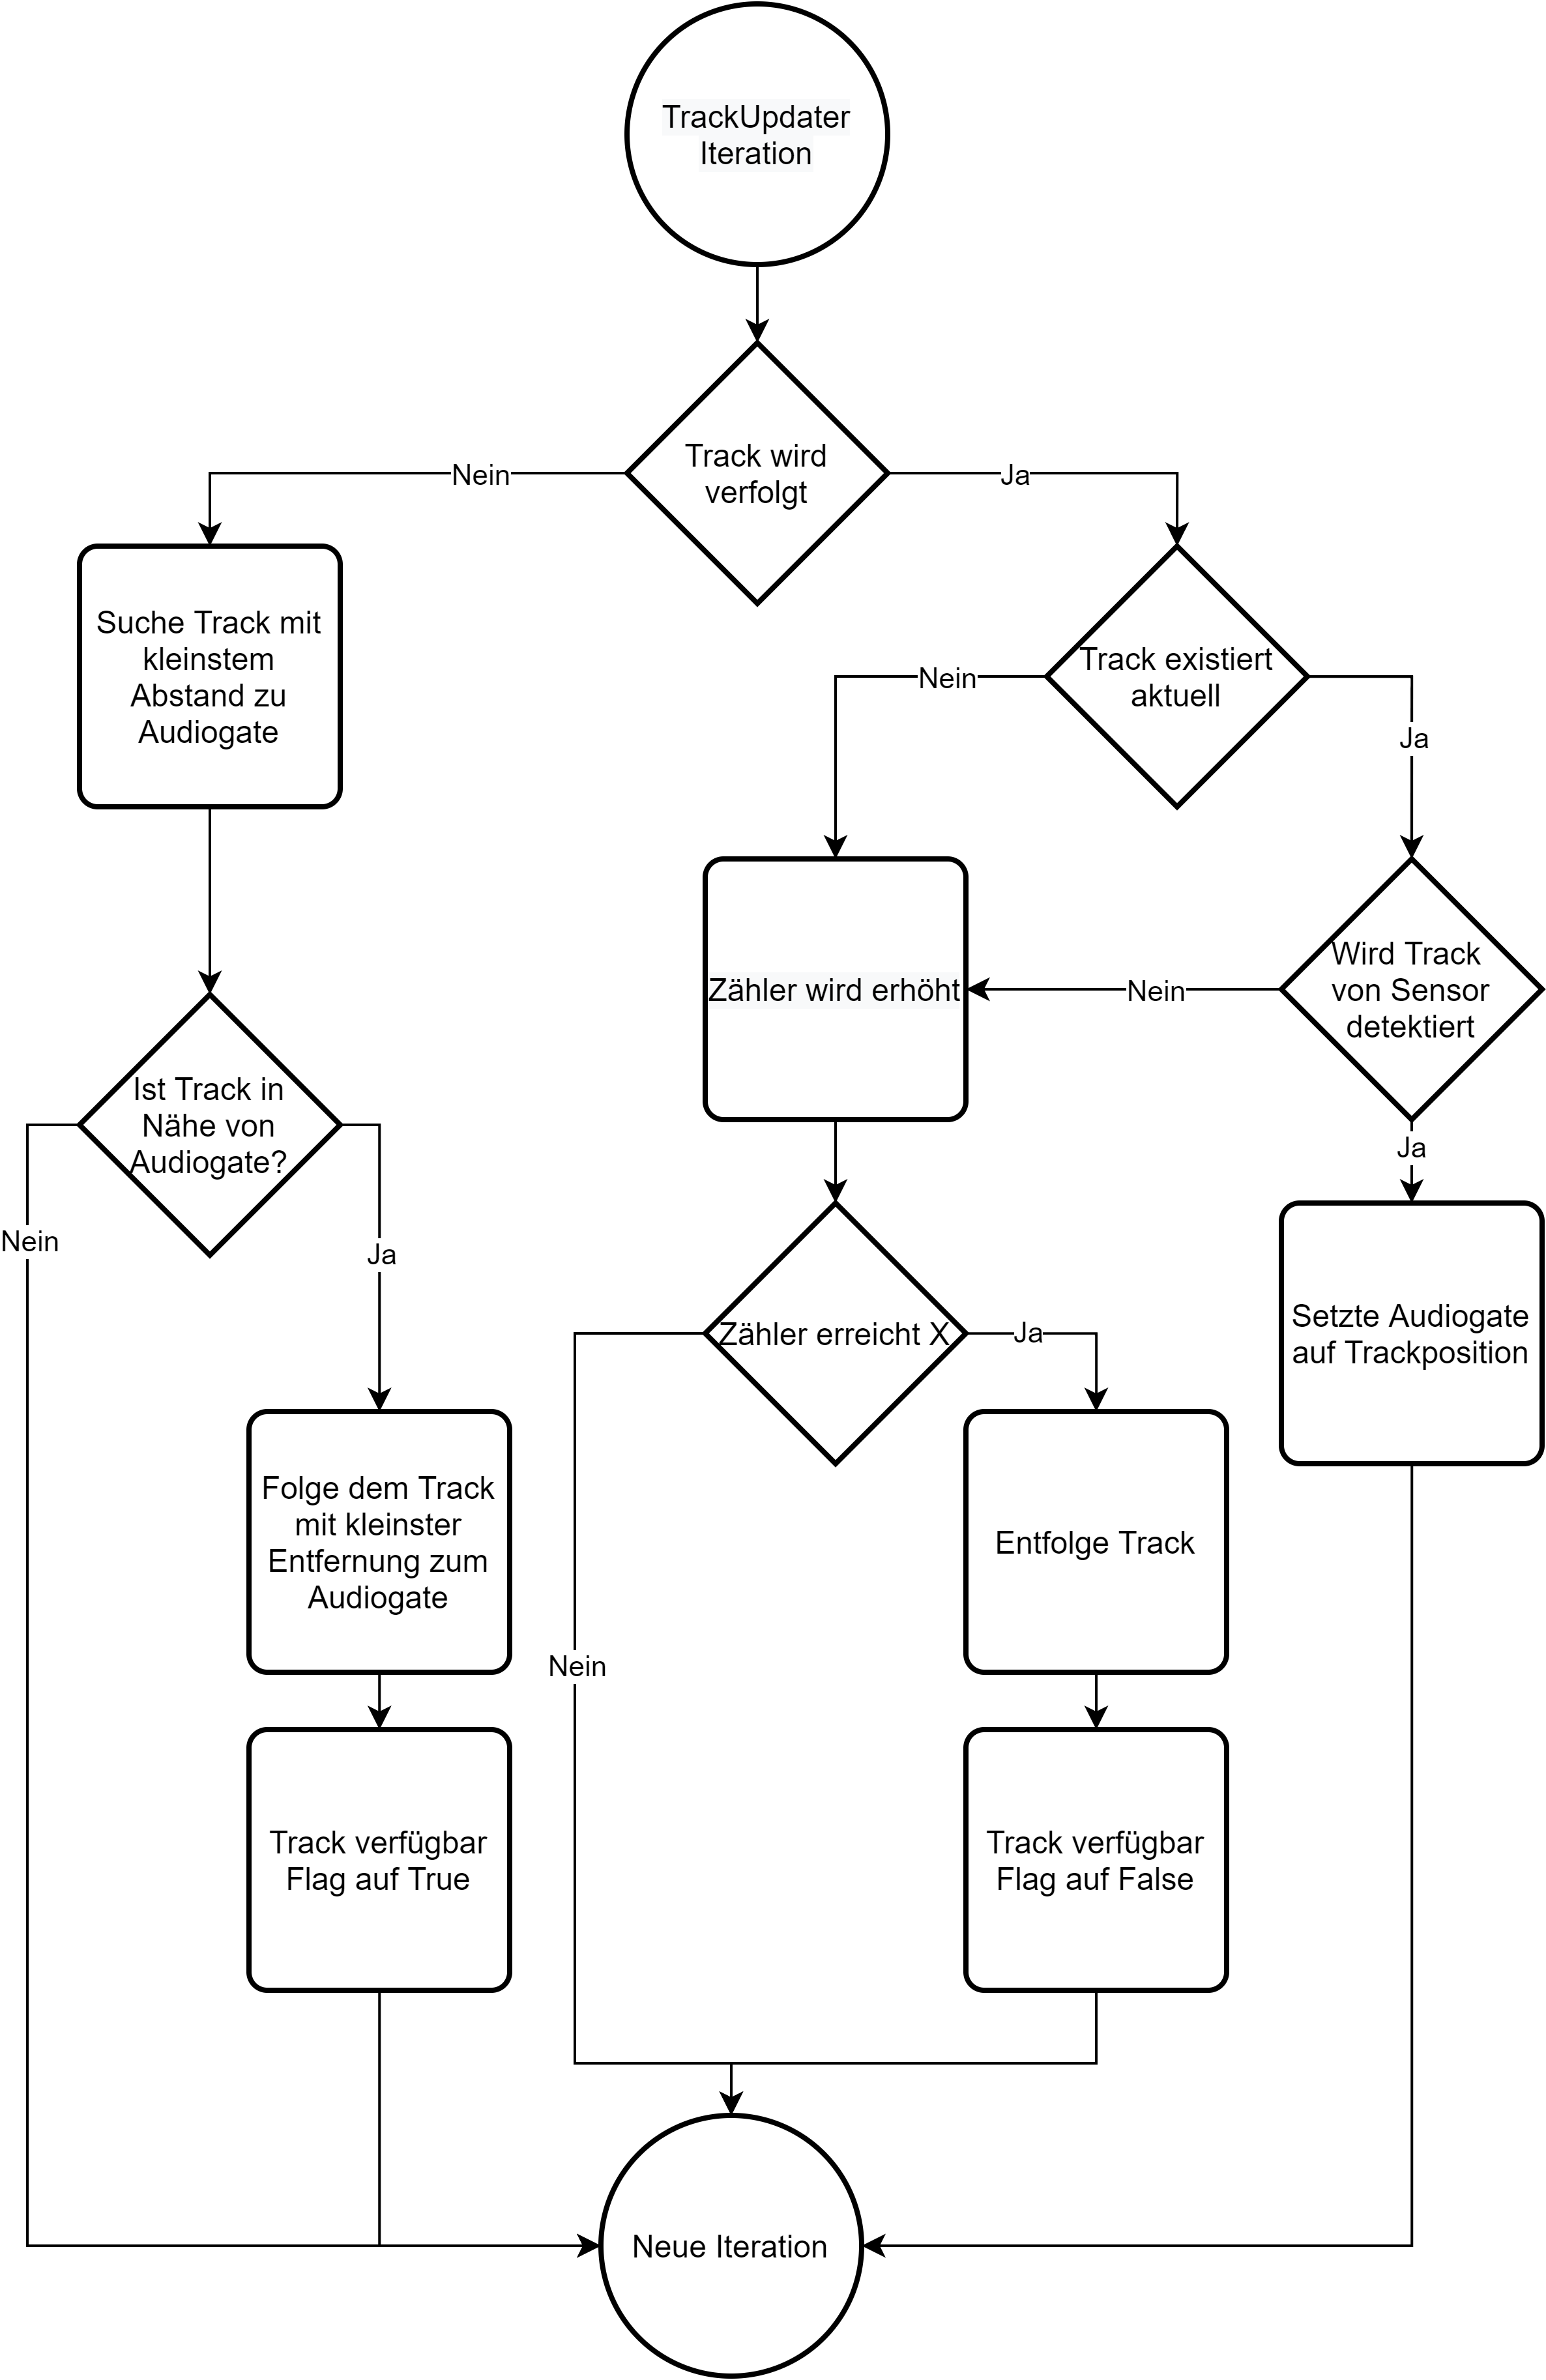
\includegraphics[width=0.65\textwidth]{content/assets/TrackUpdaterSTT.png}
    \caption{Flussdiagramm des Algorithmus des Trackupdaters}
\end{figure}



\appendix
\bibliography{quellen}{}
\bibliographystyle{plain}

\end{document}

